\documentclass{beamer}
%\usetheme[footline=infoline,headline=secheader]{UPB}
%\usetheme[footline=infoline,headline=structure]{UPB}
%\usetheme[headline=secheader]{UPB}
%\usetheme[headline=structure]{UPB}
%\usetheme[footline=infoline]{UPB}
%\usetheme{UPB} % defaults are footline=empty,headline=empty
%\usetheme{Antibes}
\usetheme{upb}
\setbeamertemplate{bibliography item}[text]
\usepackage[utf8]{inputenc}
\usepackage{hyperref}
\usepackage[ngerman]{babel}
\author[C.Robbert, P. Stilow]{Christoph Robbert, Peter Stilow}
\institute[Uni Paderborn]{Universität Paderborn}
\title[WLAN Security]{WLAN Security}
\begin{document}
\begin{frame}
\maketitle
\end{frame}

\section{Übersicht}
\begin{frame}
\frametitle{WLAN}
Grundlagen:
\begin{itemize}
	\item Direkte Kommunikation (AdHoc)
	\item Access Point (AP)
	\item Frequenzen 2,4 - 2,4835 GHz und 5,15 - 5,725 GHz
	\item Weiter Empfangsbereich
\end{itemize}
Probleme:
\begin{itemize}
	\item Abhören / Daten einspeisen
	\item Kollisionen mit anderen WLANs (oder Störsender)
	\item (Automatische) Verbindung zu offenen (gefälschten) Access Points
\end{itemize}
\end{frame}

\begin{frame}
\frametitle{WLAN}
Sicherheit
\begin{itemize}
	\item Offen (Keine Verschlüsselung)
	\begin{itemize}
		\item z.B. mit VPN verknüpfen
	\end{itemize}
	\item Verschlüsselt
	\begin{itemize}
		\item WEP (802.11)
		\begin{itemize}
			\item shared key
		\end{itemize}
		\item WPA/WPA2 (802.11i)
		\begin{itemize}
			\item Zusatz WPS
		\end{itemize}
	\end{itemize}
\end{itemize}
\end{frame}

\section{WEP}
\begin{frame}
\frametitle{WEP - Wired Equivalent Privacy}
\begin{figure}
	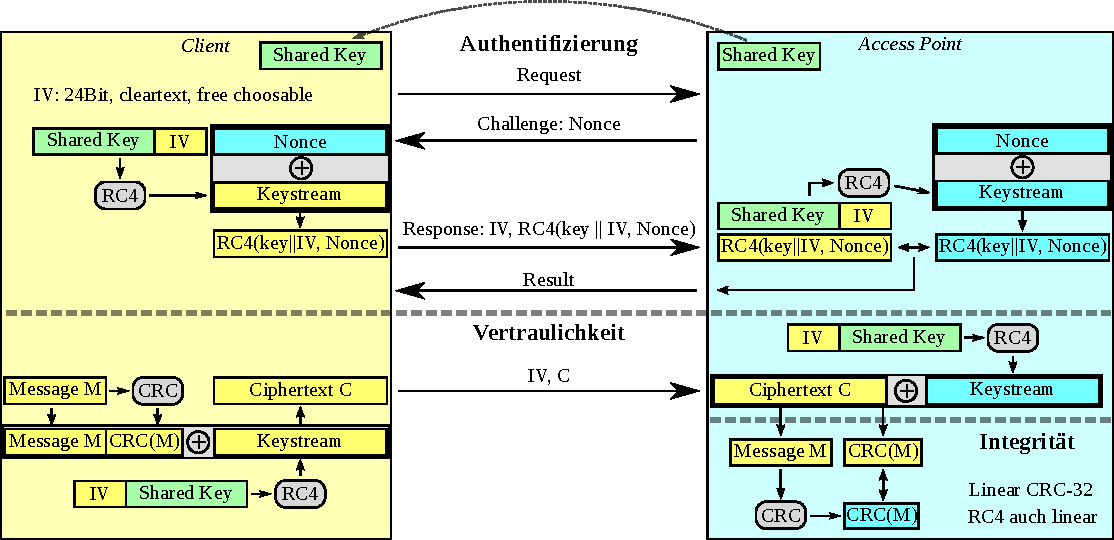
\includegraphics[width=1.0\linewidth]{figures/WEP_complete.pdf}
\end{figure}
\end{frame}


\section{Attacken gegen WEP}
\begin{frame}
\frametitle{Probleme WEP}
\begin{block}{Shared WEP Schlüssel}
\begin{itemize}
	\item manueller Austausch
	\item kein Schutz von innen
	\item 40bit
\end{itemize}
\end{block}
\begin{block}{Algorithmen}
\begin{itemize}
	\item IV 24bit, start bei 0, kein Wechsel erzwungen
	\begin{itemize}
		\item WEPplus
	\end{itemize}
	\item Lineare Zeit zum knacken des Schlüssels
	\item RC4/CRC linear
\end{itemize}
\end{block}
\end{frame}

\begin{frame}
\frametitle{WEP Angriffe}
\begin{figure}
	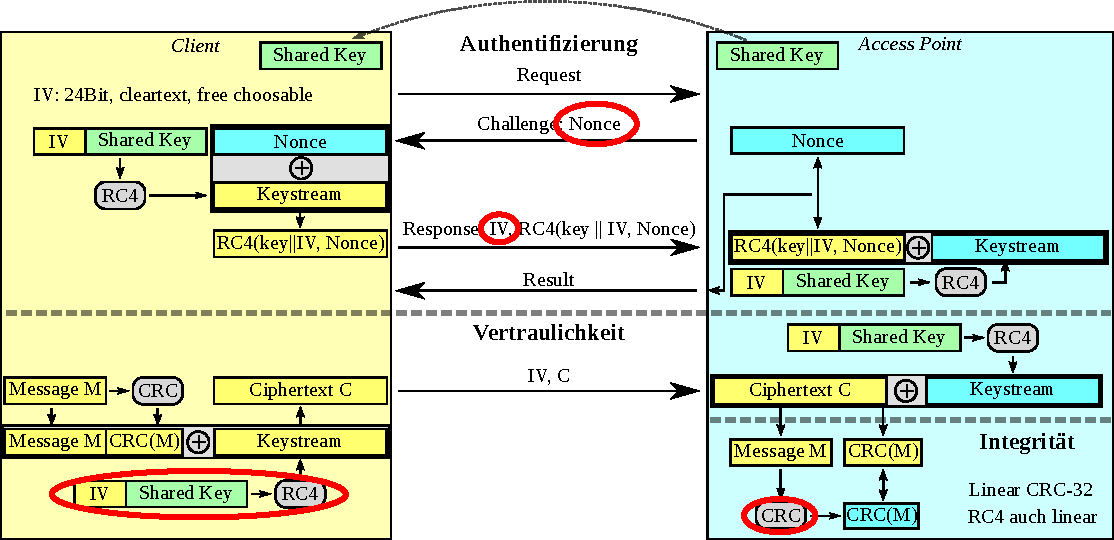
\includegraphics[width=1.0\linewidth]{figures/WEP_complete_attacks.pdf}
\end{figure}
\end{frame}

\begin{frame}
\frametitle{WEP Angriffe}
\begin{block}{WEP key knacken (ARP Pakete)}
\begin{itemize}
	\item Fluhrer-Mantin-Shamir $\rightarrow$ KoreK $\rightarrow$ Pyshkin-Tews-Weinmann
	\item Fragmentation Attack (pseudo random generation algorithm)
	\item Hirte Attack (fake AP to client)
\end{itemize}
\end{block}
\begin{block}{Nachricht entschlüsseln}
\begin{itemize}
	\item KoreK chopchop
\end{itemize}
\end{block}
\end{frame}

\section{WPA / 802.11i(WPA2)}
\begin{frame}
\frametitle{WPA / 802.11i(WPA2)}
\begin{itemize}
	\item Keines der Schutzziele von WEP (Authentizität, Vertraulichkeit, Integrität) wird erfüllt
	\item[$\Rightarrow$] Entwicklung von WPA / 802.11i(WPA2)
\end{itemize}
\begin{block}{802.11i}
\begin{itemize}
	\item Schlüsselverwaltung:
	\begin{itemize}
		\item Personal/ Pre-Shared Key (PSK)
		\item Enterprise (802.1X)
	\end{itemize}
	\item Sicherheitsprotokolle:
	\begin{itemize}
		\item TKIP(WPA, optional WPA2)
		\item AES-CCMP(optional WPA, WPA2)
	\end{itemize}
\end{itemize}
\end{block}
\end{frame}

\begin{frame}
	\frametitle{Authentifizierung mit 802.1X in 802.11i}
	\begin{itemize}
		\item Verwendung bekannter port-basierter Authentifizierung wie im kabelgebundenen Layer-2
		\item[$\Rightarrow$] Unterstützung für u.a. Zertifikat- und Smartcard-basierter Authentifizierung
	\end{itemize}
	\begin{figure}
		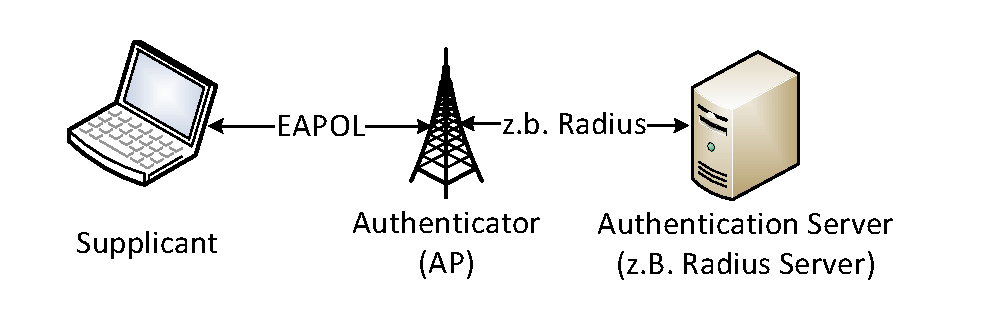
\includegraphics[scale=0.7]{figures/ap_radius.pdf}

	\end{figure}
\end{frame}

\begin{frame}
\frametitle{Schlüsselhierarchie}
	\begin{figure}
		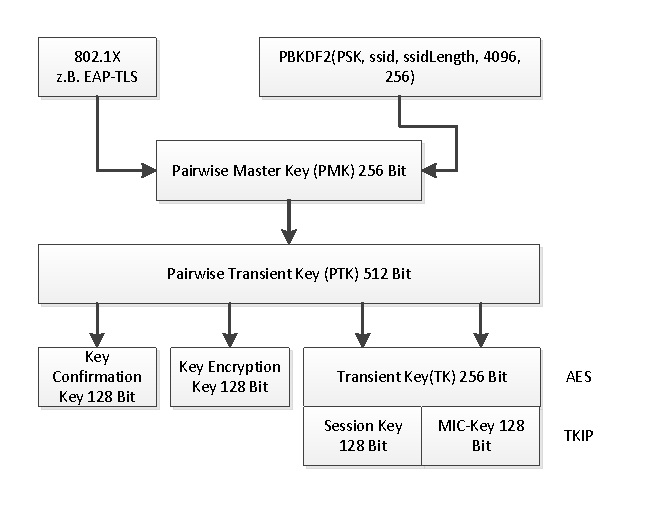
\includegraphics[scale=0.7]{figures/key_hier.pdf}
		\caption{Schlüsselhierarchie nach Abbildung 14.16 aus \cite{books/daglib/0008794}}
	\end{figure}
\end{frame}

\begin{frame}
\frametitle{4-Way-Handshake}
\begin{figure}
	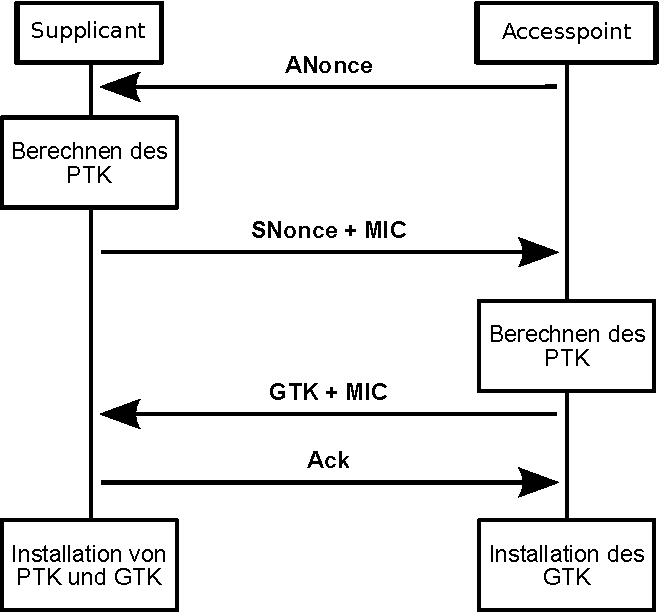
\includegraphics[width=0.5\linewidth]{figures/4-way-handshake.pdf}
	\caption{4-Way-Handshake nach \cite{ieee802.11}}
\end{figure}
\end{frame}

\begin{frame}
\frametitle{AES-CCMP}
\begin{itemize}
	\item AES-CCMP (Counter-Mode-CBC-MAC Protocol) 
	\begin{itemize}
		\item 128 Bit AES im Counter Mode (Blockchiffre)
		\item CBC-MAC stellt gleichzeitig Integrität sicher
	\end{itemize}
	\item Counter-Mode ist beweisbar sicher \cite{bellare}
\end{itemize}
\end{frame}

\begin{frame}
\frametitle{TKIP (Temporal Key Integrity Protocol)}
\begin{itemize}
	\item AES sollte in 802.11i integriert werden
	\item AES Berechnungen ist aufwendig und erforderten neue Hardware
\end{itemize}
\begin{block}{Übergangslösung TKIP}
	\begin{itemize}
		\item Erweiterung von WEP
		\item RC4 weiterhin als Basis
		\item Dynamische statt statischer Schlüssel
		\item Größere IVs:
		\begin{itemize}
			\item 48 bit statt 24 bit
			\item Benutzt als TSC(TKIP Sequence Counter)
		\end{itemize}
		\item Michael (MIC) als verbesserte Intigritätsprüfung
	\end{itemize}
\end{block}
\end{frame}

\begin{frame}
\frametitle{Schwachstellen von TKIP}
\begin{itemize}
	\item Michael hat Schwachstellen
	\begin{itemize}
		\item Brute Force Angriffe benötigen nur $2^{29}$ Packete
		\item Einzige Abwehr: Gesamten WLAN Verkehr für einige Minuten Unterbrechen
		\item[$\Rightarrow$] Ermöglicht wiederrum DoS
	\end{itemize}
	\item Wörterbuchangriff auf PBKDF2 langsam(4096 Runden HMAC-SHA1)
	\begin{itemize}
		\item Beschleunigung durch Rainbow Tables \cite{renderlab} (SSID + Passphrases)
		\item Berechnung in der Cloud \cite{cloudcracker}: 20 Minuten, 17\$, 300.000.000 Wörter
	\end{itemize}
\end{itemize}
\end{frame}


\begin{frame}
\frametitle{Hole 196}
\begin{itemize}
	\item Nur der AP darf Packete mit dem GTK verschlüsseln und an alle Clients senden
	\item Keine Überprüfung ob Packete wirklich vom AP kommen
    \item "Böser" Client nutzt den GTK um Packete an anderen Clients zu senden
	\item Kann nur von authorisierten Clienten ausgeführt werden
	\item Angriff im Standart dokumentiert
\end{itemize}
\end{frame}

\section{Andere Attacken}
\subsection{WPS}

\begin{frame}
\frametitle{WPS (Wi-Fi Protected Setup)}
Drei Endnutzerfreundliche WLAN Konfigurationsmodi:
\begin{block}{Push-Button-Connect (“PBC”)}
Benutzer drückt physischen oder virtuellen Knopf.
\end{block}
\begin{block}{PIN - Internal Registrar}
Benutzer gibt mitgelieferten WPS Pin seines Endgerätes in Webmaske des AP ein.
\end{block}
\begin{block}{PIN - External Registrar}
Benutzer bekommt Pin vom Betreiber des APs mitgeteilt und gibt ihn in sein Endgerät ein.
\end{block}
\end{frame}


\begin{frame}
\frametitle{Angriff auf WPS, PIN - External Registrar \cite{wps_attack}}
\begin{itemize}
	\item PIN ist 8 Ziffern lang
	\item Protokoll erlaubt es zu erkennen ob die ersten 4 Ziffern oder letzten 4 Ziffern falsch waren
	\item 8. Ziffer Checksumme der ersten 7 Ziffern
	\item Zu testende Kombinationen: $10^4+10^3 = 11.000$
	\item Authentification benötigt im Schnitt 1,3 Sekunden
	\item WPS Standard schreibt kein Lockdown vor. Daher selten implementiert
	\item[$\Rightarrow$] Brute Force gegen alle Kombinationen ohne Lockdown braucht circa 4 Stunden
\end{itemize}
\end{frame}

\subsection{User Tracking}
\begin{frame}
\frametitle{User Tracking}
\begin{itemize}
	\item Mülltonnen mit Werbebildschirmen und WLAN erfassten Fussgänger anhand ihrer Handies in London \cite{mulltonnen}
	\vspace{1,5cm}
	\item Endgeräte auf der Suche nach versteckten SSIDs broadcasten den Namen der versteckten SSID
	\begin{itemize}
		\item Schlechte Implementierungen broadcasten auch den Namen der bekannten unversteckten SSIDs
	\end{itemize}
\end{itemize}
\end{frame}

\section{Häufige Absicherungsempfehlungen}
\begin{frame}
\frametitle{Häufige Absicherungsempfehlungen}
\begin{block}{MAC-Filter}
Kein Nennenswerter Sicherheitsgewinn, da die MAC Adresse immer unverschlüsselt übertragen wird.
\end{block}
\begin{block}{SSID Verstecken}
AP broadcastet die SSID zwar nicht, aber sobald ein bekannter Teilnehmer sich anmeldet, wird die SSID unverschlüsselt übertragen.
\end{block} 
\begin{block}{Zufällige SSID}
Erschwert Wörterbuchattacken mit Rainbowtables gegen PBKDF2.
\end{block}
\end{frame}

\section{Tools}
\begin{frame}
\frametitle{Tools}
\begin{block}{Aircrack-ng Suite (siehe \cite{aircrack})}
	\begin{description}
		\item[aircrack-ng] WEP, WPA, WPA2-PSK Key Cracker
		\item[aireplay-ng] Erzeugt WLAN Traffic
		\item[airodump-ng] Zeichnet WLAN Rohdaten auf
		\item[airdecap-ng] Entschlüsselt aufgezeichnete WEP, WPA, WPA2 Streams
		\item[...]
	\end{description}
\end{block}
\begin{block}{FakeAP (siehe \cite{fakeap})}
Kann tausende Access Points simulieren
\end{block}
\begin{block}{Kismet (siehe \cite{kismet})/NetStumbler (siehe \cite{netstumbler})}
WLANs aufspüren und kartografieren
\end{block}
\end{frame}

\section{References}
\begin{frame}[allowframebreaks]
\frametitle{References}
\bibliographystyle{IEEEtran}
% argument is your BibTeX string definitions and bibliography database(s)
\bibliography{references}
\end{frame}
\end{document}
